
\begin{frame}\label{d.1}
\frametitle{A Theory of Dynamical Facilitation: General Idea}

\begin{columns}[T]
\begin{column}[T]{0.5\textwidth}

\begin{figure}[t]
%\includegraphics[height=0.65\textheight]{figures/pel_hopping.png}
\begin{overprint}
\vspace{-10pt}
\onslide<2>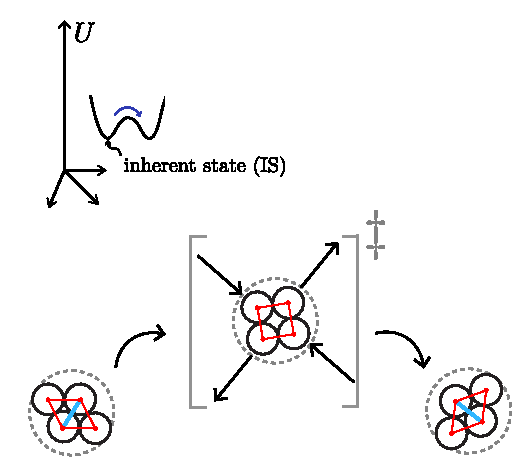
\includegraphics[width=0.975\linewidth]{1.c-fac_intro/interlude1.pdf}\caption{So far, we only discuss the first hopping event!}

\onslide<3>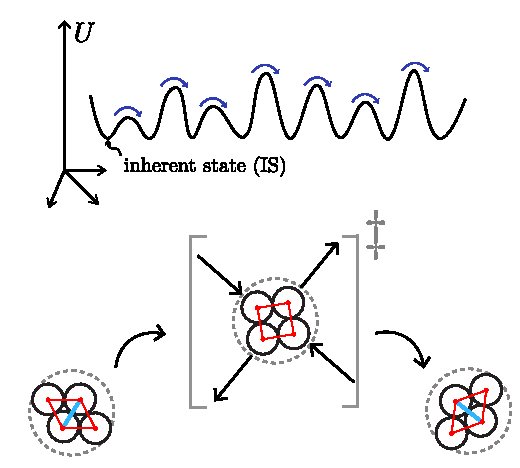
\includegraphics[width=0.975\linewidth]{1.c-fac_intro/interlude2.pdf}\caption{Relaxation involves traversing a series of ISs and energy barriers.}

\onslide<4>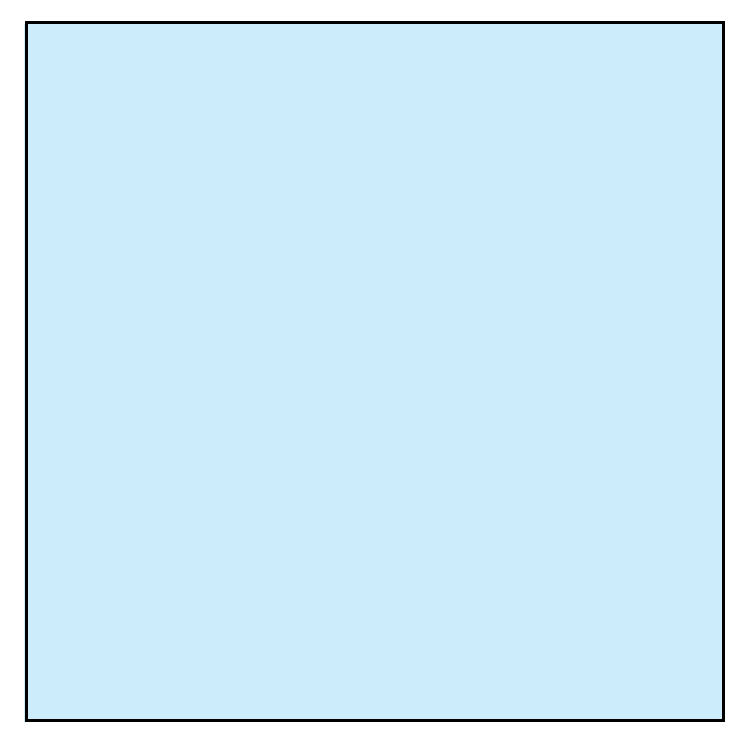
\includegraphics[width=0.95\linewidth]{1.c-fac_intro/bare_test_0.pdf}\vspace{-10pt}\caption{A system always begins with no excitations.}

\onslide<5-6>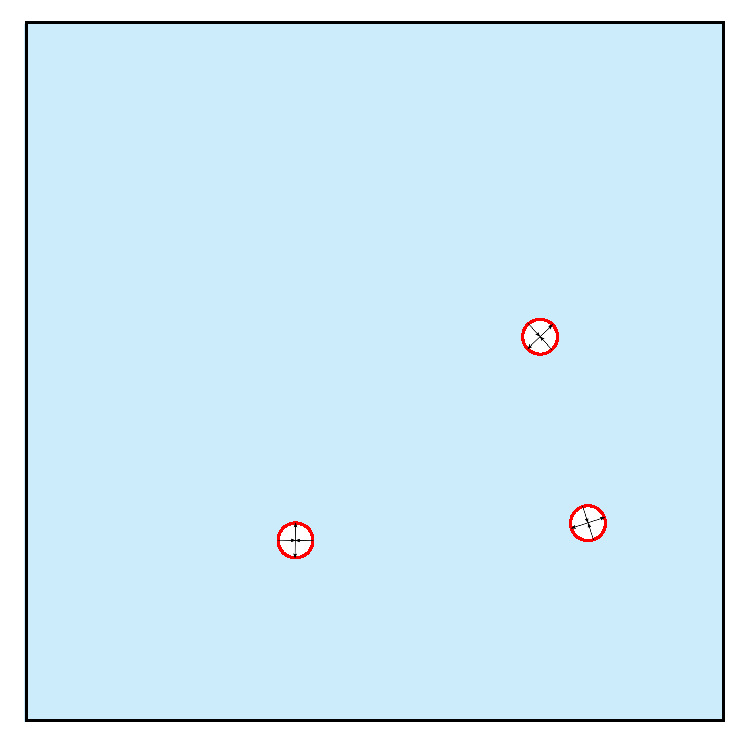
\includegraphics[width=0.95\linewidth]{1.c-fac_intro/bare_test_3.pdf}\vspace{-10pt}\caption{More excitations are created over time, anywhere in space.}

\onslide<7>\includegraphics[width=0.95\linewidth]{1.c-fac_intro/test_3.pdf}\vspace{-10pt}\caption{Excitations leave behind \textbf{elastic fields}.}

\onslide<8->\includegraphics[width=0.95\linewidth]{1.c-fac_intro/test_6.pdf}\vspace{-10pt}\caption{Elastic fields continue to accumulate until full relaxation is reached}

\end{overprint}
\end{figure}

\end{column}

\begin{column}[T]{0.5\textwidth}
\vspace{-12pt}
\begin{block}{\centering \large Origin of Facilitation}
\centering Excitations alter energy barriers for relaxation via elasticity.
{\footnotesize (Hasyim, Mandadapu,  \texttt{arXiv:2310.06584} 2023)}
%(Hasyim, Mandadapu,  \textit{J. Chem. Phys.} 155, 044504 (2021))
\end{block}

\begin{itemize}
    \item<2->Barrier for first excitation is 
    \begin{equation*}
    J_\sigma = G^\mathrm{IS} (\pi R_\mathrm{exc})^2 \epsilon_\mathrm{c}^2
    \end{equation*}
    \item<9-> Energy barrier includes interaction with the accumulated stress:
    \only<10->{
    \begin{gather*}
    J_\sigma\onslide<11->{+\km{\int \diff^2 \* x \ T_{ij}^\alpha d_{ij}^\ddagger}}
    \\
    \onslide<12->
    {d_{ij}^\ddagger: \ \text{the shear strain of the new excitation.}
    }
    \\
    \onslide<13->{T_{ij}^\alpha: \ \text{Stress at the current IS (labeled $\alpha$).}
    }
    \end{gather*}
    }
\end{itemize}

\end{column}
\end{columns}

\end{frame}
